\documentclass{beamer}

\usepackage[utf8]{inputenc}
\usepackage[spanish]{babel}
\usepackage{hyperref}
\hypersetup{pdfkeywords=colabore tabio cundinamarca 2012 taller herramientas colaborativas web wiki etherpad t2t latex altaimpedancia altaz mutabit hackbo}
\usepackage{graphicx}

\title[Herramientas colaborativas web]{Herramientas colaborativas web}
\author[JEGC 2012]{Jorge~Ernesto~Guevara~Cuenca}
\institute[\url{http://www.hackbo.co}]
{ \inst{1}
  Colibri - Comunidad de Usuarios de Software Libre en Colombia\\
  \url{http://www.slcolombia.org}
  \and
  \inst{2}
  Alta Impedancia - \url{http://www.altaimpedancia.org}
  \and
  \inst{3}
  Hackbo - Hackerspace Bogotá -  \url{http://www.hackbo.co}
}
\date[Colabore - Tabio, Cundinamarca]
{Colabore - Tabio Cundinamarca\\Laboratorio de aprendizaje colectivo\\11 de agosto de 2012}

\subject{Herramientas colaborativas web, Colabore - Tabio Cundinamarca\\Laboratorio de aprendizaje colectivo\\11 de agosto de 2012}


\logo{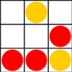
\includegraphics[height=1cm]{img/hackbo}}

\AtBeginSubsection[]
{ \begin{frame}<beamer>{Agenda}
    \tableofcontents[currentsection,currentsubsection]
  \end{frame}}

\beamerdefaultoverlayspecification{<+->}


\begin{document}

\begin{frame}
  \titlepage
\end{frame}

\begin{frame}
  \frametitle{Agenda}
  \tableofcontents
  % You might wish to add the option [pausesections]
\end{frame}

\section<presentation>*{Herramientas colaborativas web}

\begin{frame}
  \frametitle{Objetivo}
  \begin{itemize}
  \item Hacer una introducción a 2 tecnologías web para trabajo colaborativo no necesariamente en linea, una en tiempo real y otra asíncrona.
  \end{itemize}
\end{frame}

\section{Marcado}

\begin{frame}[fragile]{HTML}{Etiquetas (tags)}
\begin{verbatim}
<!DOCTYPE html>
<html>
 <body>

  <h1>Encabezado</h1>

  <p>Esto es un párrafo.</p>

 </body>
</html>
\end{verbatim}
\end{frame}

\begin{frame}{Etiquetamiento ligero}{txt2tags}
  \url{http://txt2tags.org/online.php}
\end{frame}

\section{Wikis}
\begin{frame}{Wikipedia}
  \begin{itemize}
  \item MediaWiki
  \end{itemize}
\end{frame}

\begin{frame}{El Directorio}
  \begin{itemize}
  \item MoinMoin
  \end{itemize}
\end{frame}

\section{Pads}
\begin{frame}{Etherpad}
  \begin{itemize}
  \item NodeJS
  \end{itemize}
\end{frame}


\section<presentation>*{Sobre este documento}

\begin{frame}
  \begin{block}{Licencia}
    \begin{figure}
      
\includegraphics[scale=0.9]{img/by-sa}
    \end{figure}
    \centering
    \small Creative Commons\\
    \small Atribución-Compartir Obras Derivadas Igual 2.5 Colombia\\
    \small \url{http://creativecommons.org/licenses/by-sa/2.5/co}
  \end{block}
  \begin{block}{}
    Creado con \LaTeX / Beamer
  \end{block}
\end{frame}


\end{document}
